\DiaryEntry{Touching Circles}{2020-02-10}{Maths}

This is another example how high dimensions run against our intuition. We consider a construction as shown in the following for the 2-dimensional case:

\begin{figure}[H]
\centering
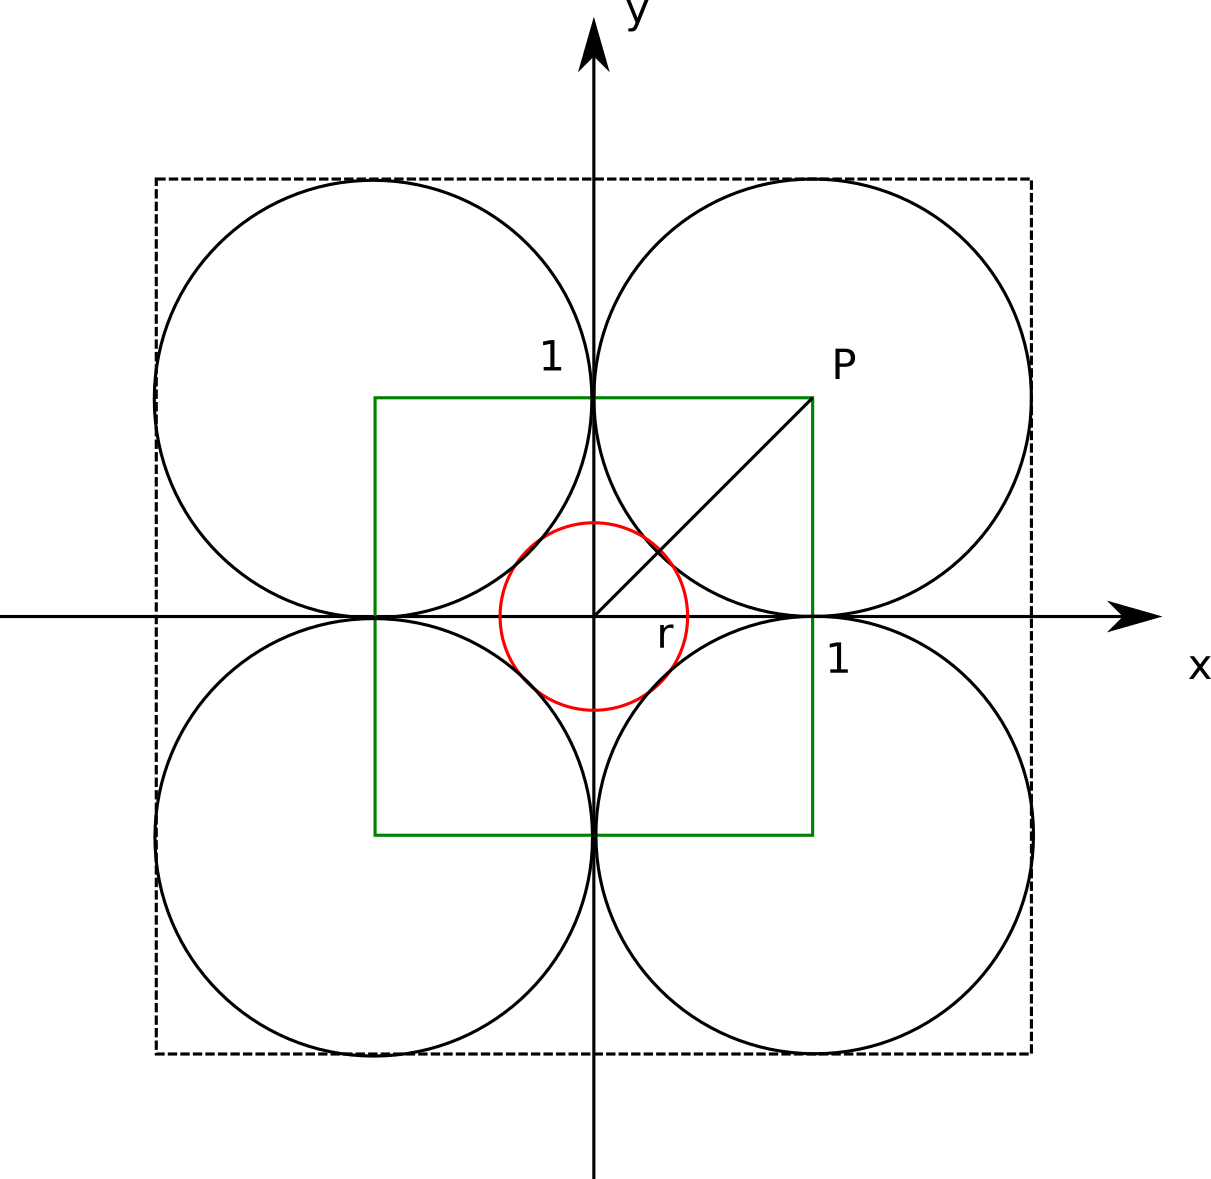
\includegraphics[scale=0.75]{images/high_dim_03_1.png}
\end{figure}

There are four circles located at $(1,1)$, $(1,-1)$, $(-1,1)$, and $(1,1)$ with radius $1$. They leave space for the small circle shown in red with center at the origin and radius $r$. How large is $r$? For symmetry reasons we consider the point $P$. The distance between the origin and $P$ is given by

\bee
d = \sqrt{1^2 + 1^2} = \sqrt{2}
\eee

Since the circles have radius $1$, this leaves

\bee
r = d - 1 = \sqrt{2} - 1 \approx 0.4142
\eee

So far, so good: The inner circle looks really much smaller, and this reflects in the value of $r$ as well. If we go up to 3 dimensions, we consider the distance from the origin to $(1,1,1)$:

\bee
d = \sqrt{1^2 + 1^2 + 1^2} = \sqrt{3}
\eee

from which we obtain

\bee
r = \sqrt{3} - 1 \approx 0.7321
\eee

From this we can deduce the expression for the general case with $N$ dimensions; we have

\bee
d = \sqrt{N}, \quad r = \sqrt{N}-1
\eee

We see that $r$ increases unbounded with dimension $N$; for $N=4$ we have $r = 1$; i.e. the inner circle has the same size as the outer circles. It therefore touches the green box. Going to even higher dimensions, things go a little bit out of hand; for $N=10$, we have $r \approx 2.1623$. This is weird, as it is \emph{larger} than the bounding box of the whole construction shown in dashed lines! 


%%% Local Variables:
%%% mode: latex
%%% TeX-master: "journal"
%%% End:
